% !TeX spellcheck = en_GB
%%=============================================================================
%% Methodologie
%%=============================================================================

\chapter{\IfLanguageName{dutch}{Methodologie}{Methodology}}
\label{ch:methodologie}
% Tip: Begin elk hoofdstuk met een paragraaf inleiding die beschrijft hoe dit hoofdstuk past binnen het geheel van de bachelorproef. Geef in het bijzonder aan wat de link is met het vorige en volgende hoofdstuk.

% TODO: Hoe ben je te werk gegaan? Verdeel je onderzoek in grote fasen, en licht in elke fase toe welke stappen je gevolgd hebt. Verantwoord waarom je op deze manier te werk gegaan bent. Je moet kunnen aantonen dat je de best mogelijke manier toegepast hebt om een antwoord te vinden op de onderzoeksvraag:

% What are the advantages and disadvantages of a migration from Windows Server 2016 to 2019 in a business environment?
%% What are the differences between the standard, ServerCore and Nano version of Windows Server 2019? Deze zijn virtualizatiecontainers!
%% Can we migrate SAP from an existing Windows Server 2016 to 2019 in a business environment?
%% How can the new features of Windows Server 2019 be leveraged in the migrated infrastructure? 

In this chapter the upgrade from Windows Server 2016 to Windows Server 2019 will be researched. This upgrade will first be performed using the in-place upgrade method after which the process will be repeated using a migration. After this the migration of a typical SAP environment, as described by Delaware, from Windows Server 2016 to Windows Server 2019 will be examined. To continue the different versions of the container images will be analysed and how these can lower virtual machine overhead, and improve virtualization efficiency. Finally, their will be a discussion about how the new features that come with Windows Server 2019 can be leveraged in the migrated infrastructure. But first the used infrastructure will be discussed.

\section{Technical specifications of the proof of concept setup}
The proof of concept was made on a bare-metal server running Windows Server 2016. The proof of concept environment was than virtualized using Hyper-V. 
\begin{itemize}
	\item CPU: Intel Xeon E5620
	\item RAM: 96 GB 
	\item HDD: 500 GB
	\item OS Version: Windows Server 2016
	\item Hyper-V role installed
	\item Administrative rights on the device
\end{itemize}
The proof of concept environment was based on the Modern Desktop Deployment and Management Lab Kit provided by Microsoft. \autocite{Gallagher2018}
This to make replication of the proof of concept simple and efficient.
\\
The Modern Desktop Deployment and Management Lab Kit consists of the following components:
\\

\begin{table}[ht]
	\centering
	\begin{adjustbox}{width=1\textwidth}
	\begin{tabular}{l|l}
		Server Name  & Roles \& Products                                                  	 \\ 
		\hline
		HYD-DC1      & Active Directory Domain Controller, DNS, DHCP, Certificate Services 	   \\
		HYD-MDT1     & Microsoft Deployment Toolkit                                        		\\
		& Windows 10 1809 ADK                                                 					 \\
		& Windows Deployment Services                                         					  \\
		HYD-CM1      & System Center Configuration Manager 1806                            		   \\
		& Windows Deployment Services                                         						\\
		& Microsoft Deployment Toolkit                                         						 \\
		& Windows 10 1809 ADK                                                 			 			  \\
		& Windows Software Update Services                                        		  			   \\
		& Microsoft SQL Server 2014                                           						    \\
		HYD-APP1     & Microsoft BitLocker Administration and Monitoring                   				 \\
		& Microsoft SQL Server 2014                                          							  \\
		HYD-GW1      & Remote Access for Internet Connectivity                           				   \\
		HYD-INET1    & Simulated Internet                                                			 	    \\
		HYD-VPN1     & Remote Access for VPN                                             				     \\
		HYD-CLIENT1  & Windows 10 1809 Domain Joined                                  					      \\
		& Office 365 ProPlus Build 16.0.11121.20000                         								   \\
		HYD-CLIENT2  & Windows 10 1809 Domain Joined                                     					    \\
		& Office 365 ProPlus Build 16.0.11121.20000                           									 \\
		HYD-CLIENT3  & Windows 10 1809 Workgroup                                         						  \\
		HYD-CLIENT4  & Windows 10 1809 Workgroup                                          						   \\
		HYD-CLIENT5 & Bare metal (no installations)                                      						    \\
		HYD-CLIENT6 & Bare metal (no installations)                                       							 \\
		HYD-CLIENT7  & Windows 7 Domain Joined                                            
	\end{tabular}
	\end{adjustbox}
	\caption[Lab Kit Components]{Modern Desktop Deployment and Management Lab Kit Components}
	\scriptsize	
	Adapted from \cite{MicrosoftCorporation2019}
	%TODO Bronvermelding correct?
	\label{tab:MDDMLK2016}
\end{table}

	
Only HYD-CLIENT1 will be kept in the proof of concept. Connection to the other \acrshort{vm}s can be made using the following credentials:
\begin{table}[ht]
	\centering
	\begin{adjustbox}{width=1\textwidth}
	\begin{tabular}{l|lll}
		User                 & Access Type              & User Name                    & Password \\
		\hline
		Local Administrator  & Administrative           & Administrator                & P@ssw0rd \\
		Domain Administrator & Enterprise Administrator & CORP\textbackslash{}LabAdmin & P@ssw0rd
	\end{tabular}
	\end{adjustbox}
	\caption[Lab Kit Credentials]{Modern Desktop Deployment and Management Lab Kit Credentials}
	\scriptsize	
	Adapted from \cite{MicrosoftCorporation2019}
	%TODO Bronvermelding correct?
	\label{tab:MDDMLK2016}
\end{table}

\section{Upgrading the \acrshort{os}}
\subsection{In-place upgrade to Windows Server 2019}
In this subsection an in-place upgrade will be performed on the \acrfull{dc} from Windows Server 2016 to Windows Server 2019. To continue the operation of the applications running on the \acrshort{dc} and the connections to the other servers in the domain will be verified. Possible problems and solutions will be discussed as they reveal themself.
% Only upgrading DC and testing if it brakes something in the Lab Kit.
% In-Place Upgrade does not work with evaluation
\subsubsection{Prerequisites}
Before starting the upgrade it is important to verify that the server is backed-up. Be sure to check when the last back-up was performed and if one has ever been succesfully restored. After this it is important to verify that all the third-party applications on the server are supported by the newest version of the \acrshort{os}. Finally, the forest and domain need to be prepared for the upgrade. The installation media provides tools for this. The following code completes this process. Be sure to verify the mounting point of the installation media, in this scenario it has been mounted to D:\textbackslash .

\begin{lstlisting}
	:d
	cd support\adprep
	adprep /forestprep
	adprep /domainprep
\end{lstlisting}
\begin{figure}[h]
	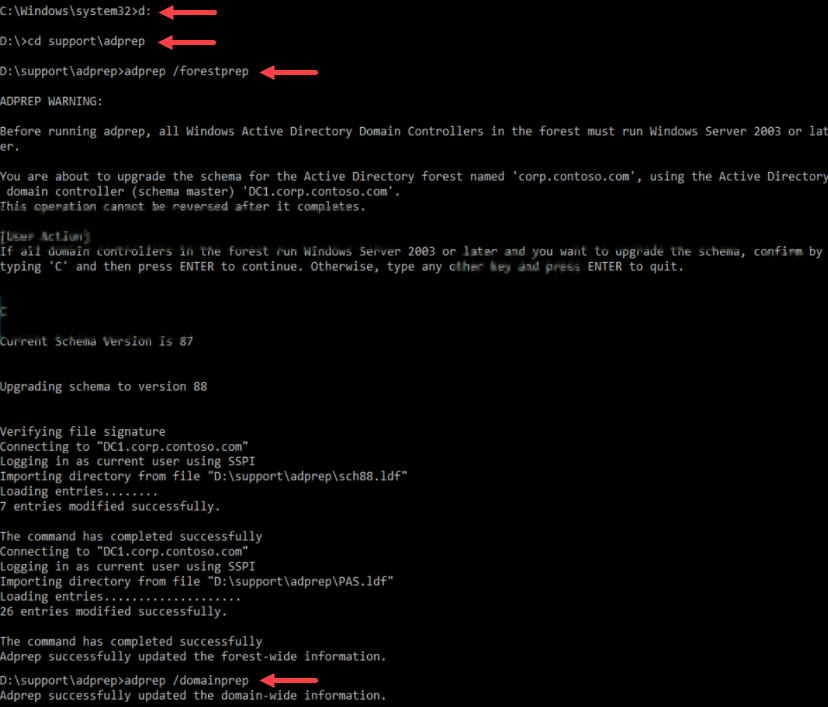
\includegraphics[height=8cm]{img/In-Place_WS_1.png}
	\captionsetup{width=0.8\linewidth}
	\centering		
	\caption{Preparing the forest and domain}
	\label{fig:inplace1}
\end{figure}

\subsubsection{In-place upgrade}
After the previous step the setup from the installation is to be launched. From this point on the upgrade process has been visualised through the figures below. If there is no image present of the current screen it is expected to click next and continue the in-place upgrade. Be sure to not use the evaluation version of Windows Server 2019, since this does not support in-place upgrades.
\begin{figure}[h]
	\begin{subfigure}{0.5\textwidth}
		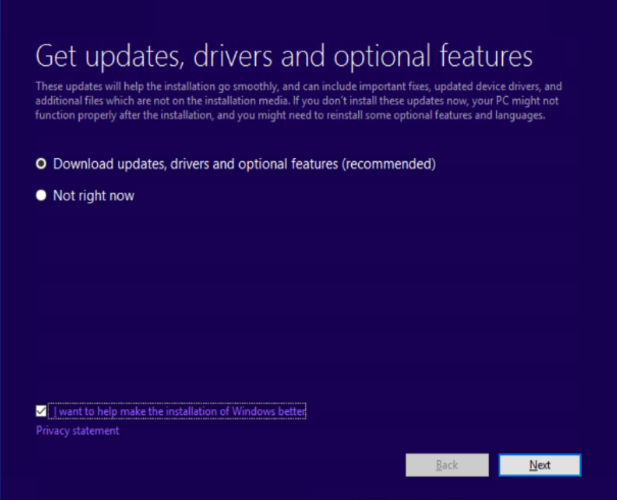
\includegraphics[width=0.9\linewidth,height=4.3cm]{img/In-Place_WS_2.png}
		\captionsetup{width=0.8\linewidth}
		\centering		
		\caption{Click next to upgrade}
		\label{fig:inplace2}
	\end{subfigure}
	\begin{subfigure}{0.5\textwidth}
		\captionsetup{width=0.8\linewidth}
		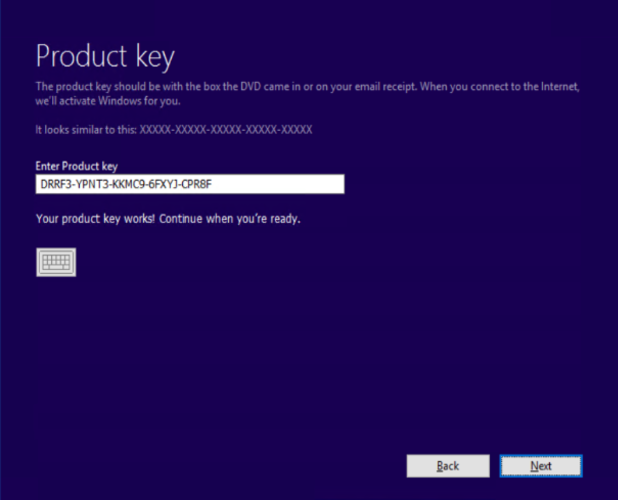
\includegraphics[width=0.9\linewidth,height=4.3cm]{img/In-Place_WS_3.png}
		\centering
		\caption{Enter the product key}
		\label{fig:inplace3}
	\end{subfigure}
\end{figure}
\begin{figure}[h]\ContinuedFloat
	\begin{subfigure}{0.5\textwidth}
		\captionsetup{width=0.8\linewidth}
		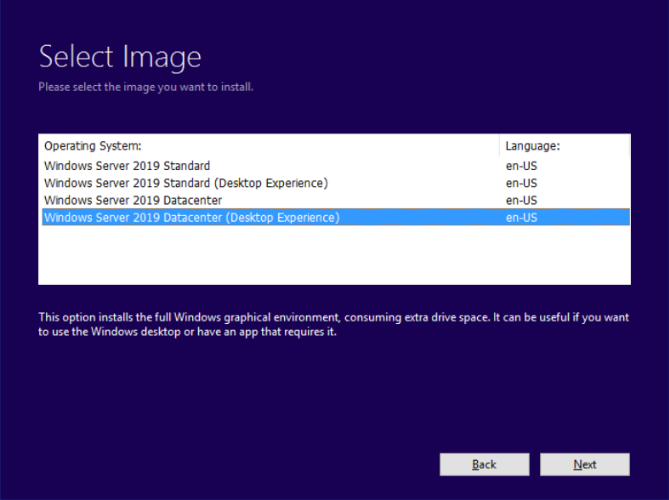
\includegraphics[width=0.9\linewidth,height=4.3cm]{img/In-Place_WS_4.png} 
		\centering
		\caption{Select a version of choice}
		\label{fig:inplace4}
	\end{subfigure}
	\begin{subfigure}{0.5\textwidth}
		\captionsetup{width=0.8\linewidth}
		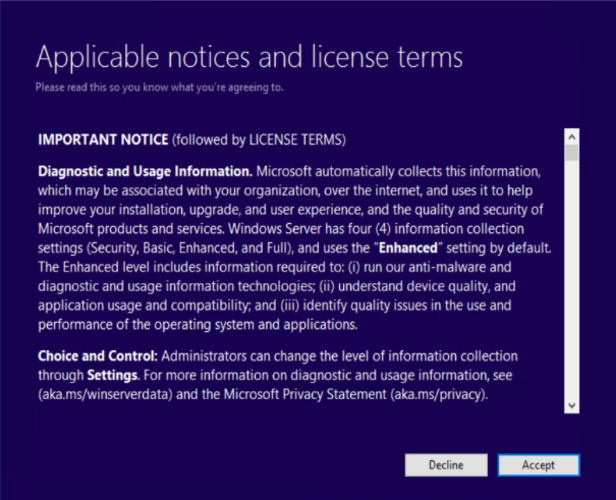
\includegraphics[width=0.9\linewidth,height=4.3cm]{img/In-Place_WS_5.png}
		\centering
		\caption{Accept the licence terms}
		\label{fig:inplace5}
	\end{subfigure}
\end{figure}
\begin{figure}[h]\ContinuedFloat
	\begin{subfigure}{0.5\textwidth}
		\captionsetup{width=0.8\linewidth}
		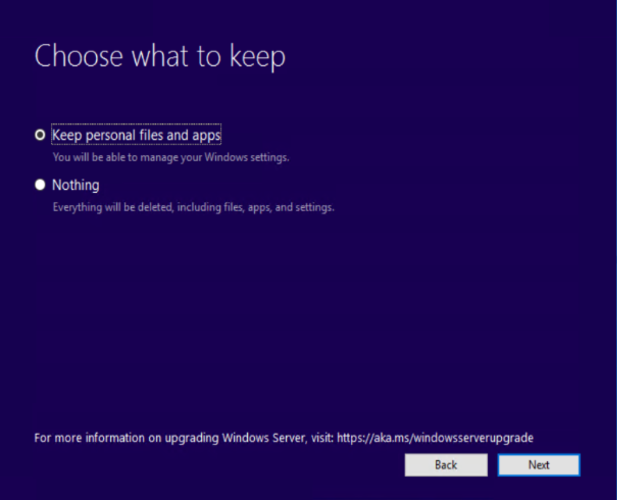
\includegraphics[width=0.9\linewidth,height=4.3cm]{img/In-Place_WS_6.png} 
		\centering
		\caption{Select "Keep personal files and apps" to perform an in-place upgrade}
		\label{fig:inplace6}
	\end{subfigure}
	\begin{subfigure}{0.5\textwidth}
		\captionsetup{width=0.8\linewidth}
		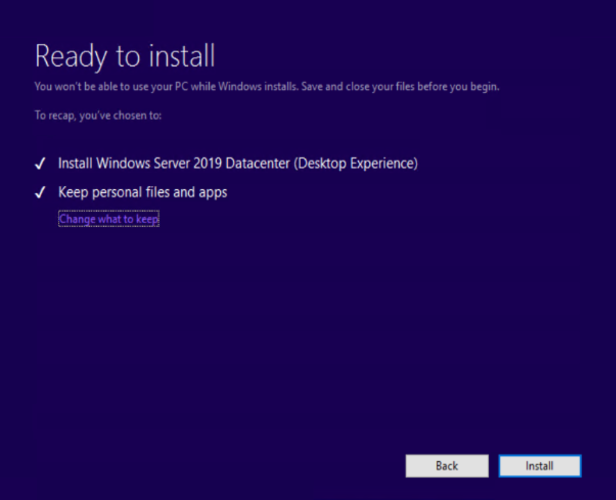
\includegraphics[width=0.9\linewidth,height=4.3cm]{img/In-Place_WS_7.png}
		\centering
		\caption{Review the settings and start the installation}
		\label{fig:inplace7}
	\end{subfigure}
	\caption{The in-place upgrade process}
	\label{fig:inplace}
\end{figure}
\subsubsection{Verification}
% nltest /sc_query:corp.contoso.com
\subsection{Migration to Windows Server 2019}
\subsubsection{Prerequisites}
\subsubsection{Migration}
\subsubsection{Verification}
\subsection{Conclusion}
% TODO https://raw.githubusercontent.com/coreyp-at-msft/ws-upgrade-center/dev/en-US/media/upgrade-paths-2-small.png
% Explain how 2016 -> 2019 is easy but previous version can require consecutive upgrades that each bring their own "bagage"
\section{SAP migration}
\subsection{Technical specifications of SAP environment}
\subsection{Migration of SAP}
\section{Windows, Windows Server Core and Nano Server}